\chapter{Sprint 05 – Déploiement de la plateforme}
\section*{Introduction}

Le Sprint 05 marque l’ultime étape du projet : le déploiement de l’application Swift Helpers dans un environnement de production stable, sécurisé et accessible à distance. Ce sprint a pour objectif de regrouper tous les modules développés (clients, prestataires, administration, ordres de mission) dans une architecture Dockerisée, orchestrée par \texttt{docker-compose}.

Le processus de déploiement comprend également la configuration d’un reverse proxy avec NGINX, la gestion de la base de données PostgreSQL, ainsi que la sécurisation des accès via un certificat SSL. L’ensemble est hébergé sur un serveur VPS avec nom de domaine personnalisé.

Les tâches de ce sprint ont permis d’assurer :
\begin{itemize}
  \item L’automatisation du déploiement via Docker et docker-compose ;
  \item La configuration réseau (ports, reverse proxy, volumes) entre les différents conteneurs ;
  \item L’exposition de l’application sur Internet avec HTTPS ;
  \item La portabilité et la reproductibilité de l’environnement.
\end{itemize}


\section*{Backlog du Sprint 05}
\begin{table}[H]
\centering
\begin{tabular}{|c|p{5cm}|c|p{5.5cm}|c|c|}
\hline
\textbf{ID US} & \textbf{User Story} & \textbf{ID Task} & \textbf{Tâche} & \textbf{Estimation} & \textbf{Responsable} \\
\hline

US05.01 & En tant qu’admin technique, je veux pouvoir déployer toute l’application dans un environnement de production.
        & T05.01.1 & Préparer les Dockerfile pour Angular et Django & 2h & Aziz \\
        \cline{3-6}
        & & T05.01.2 & Configurer docker-compose (base de données, frontend, backend) & 2h & Aziz \\
        \cline{3-6}
        & & T05.01.3 & Configuration Nginx + proxy inverse & 2h & Aziz \\
        \cline{3-6}
        & & T05.01.4 & Mise en production sur serveur distant (VPS) & 2h & Aziz \\
\hline

US05.02 & En tant qu’utilisateur, je peux accéder à l'application via une URL sécurisée.
        & T05.02.1 & Configuration du nom de domaine et certificat SSL (Let's Encrypt) & 1h & Aziz \\
\hline

\end{tabular}
\caption{Sprint Backlog – Déploiement de la plateforme}
\end{table}

\section{Introduction à Docker et à l’orchestration de conteneurs}

\subsection*{Qu’est-ce que Docker ?}
Docker est une technologie de virtualisation légère qui permet d’emballer une application et toutes ses dépendances dans un conteneur exécutable sur n’importe quel environnement. Contrairement aux machines virtuelles, les conteneurs Docker utilisent le même noyau que l’hôte, ce qui les rend beaucoup plus rapides et efficaces.

\begin{itemize}
  \item \textbf{Portabilité} : le code s’exécute de la même manière en local ou en production.
  \item \textbf{Isolation} : chaque service (Angular, Django, PostgreSQL) fonctionne dans un conteneur indépendant.
  \item \textbf{Déploiement simplifié} : les conteneurs sont orchestrés via \texttt{docker-compose}.
\end{itemize}

\section{Architecture de déploiement}

\noindent L’architecture cible repose sur une séparation claire des composants :
\begin{itemize}
  \item \textbf{Frontend Angular} : compilé et servi via un conteneur Nginx.
  \item \textbf{Backend Django} : API exposée via Gunicorn + gestion des WebSockets avec Django Channels.
  \item \textbf{Base PostgreSQL} : conteneur de base de données relationnelle.
  \item \textbf{Reverse Proxy Nginx} : pour acheminer les requêtes HTTP/S et WebSocket.
\end{itemize}

\begin{figure}[H]
\centering
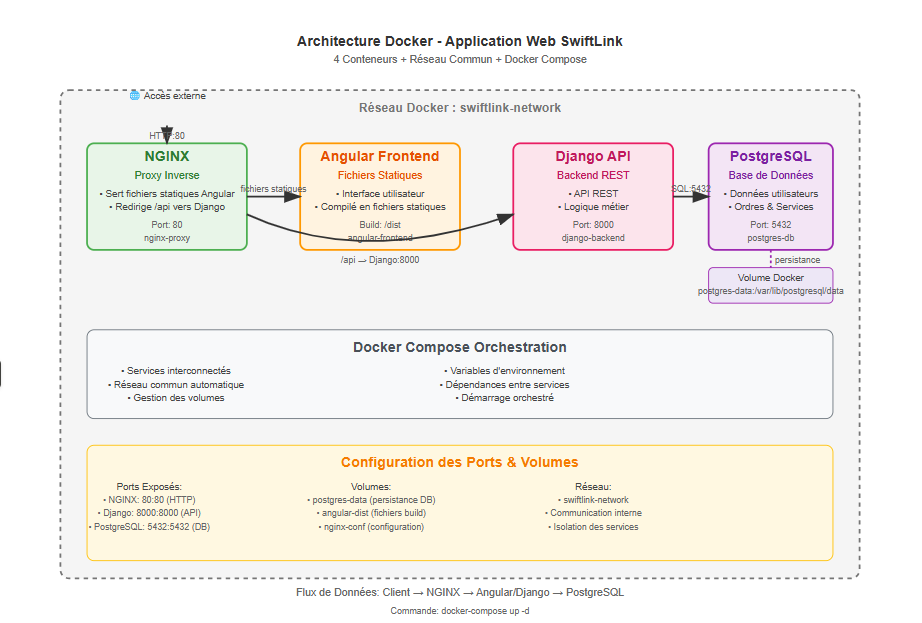
\includegraphics[width=0.9\linewidth]{figures/architecture docker.png}
\caption{Architecture de déploiement multi-conteneurs avec Docker}
\end{figure}

\section{Configuration Docker}

\subsection*{Dockerfile – Backend (Django)}
\textit{Ce fichier construit une image contenant Django, les dépendances Python et le serveur Gunicorn.}

\subsection*{Dockerfile – Frontend (Angular)}
\textit{Ce fichier compile le projet Angular avec \texttt{ng build --prod} et copie les fichiers statiques dans une image Nginx.}

\subsection*{docker-compose.yml}
\textit{Décrit et orchestre les services \texttt{frontend}, \texttt{backend}, \texttt{db} et \texttt{nginx}. Chaque service est isolé, mais peut communiquer via un réseau interne Docker.}

\section{Mise en production}

\subsection*{Configuration Nginx}
\begin{itemize}
  \item Rediriger les requêtes Angular vers l’index HTML
  \item Acheminer les requêtes API vers Django (port 8000)
  \item Gérer les WebSocket (Channels, via Daphne)
\end{itemize}

\subsection*{Nom de domaine et sécurité}
\begin{itemize}
  \item Enregistrement DNS du domaine
  \item Installation de certificat SSL avec Certbot
  \item Redirection automatique HTTP → HTTPS
\end{itemize}

\subsection*{Accès public à la plateforme}
\textit{Une fois déployée, la plateforme est accessible à l’URL :}

\begin{center}
\texttt{https://www.swift-helpers.com}
\end{center}

\section*{Conclusion}
\textit{Ce sprint final marque la mise en ligne complète du système. Grâce à Docker, le processus est reproductible, automatisé et sécurisé. Le système est désormais accessible aux utilisateurs finaux dans un environnement stable.}

\section*{Conclusion}

Grâce à ce sprint, l’application Swift Helpers est désormais opérationnelle en ligne, prête à être utilisée par les utilisateurs finaux. L’environnement de production déployé garantit une infrastructure stable, isolée, sécurisée et facilement maintenable.

Le recours à Docker et à l’orchestration avec docker-compose a permis de standardiser le processus de mise en ligne, de minimiser les erreurs de configuration, et de faciliter les futures évolutions ou mises à jour de la plateforme.

Cette phase de déploiement clôture le cycle de développement logiciel en assurant la transition entre l’environnement de développement local et l’environnement d’exploitation réel. Elle ouvre la voie à l’exploitation effective de la solution, à la supervision des usages et aux futurs cycles d’amélioration continue.
